\section{\acs{etl}-Strecke} \label{etlpipeline}

Für den Import der Information der \ac{icd10gm} in der \ac{db} wurde eine \ac{etl}-Strecke entwickelt. Dazu wurden \ac{bash}-Skripts unter Ubuntu 20.04 programmiert und durchgeführt. 

--Warum \ac{bash}?

Die Anfang Punk für die Durchführung der \ac{etl} sind die \ac{zip}-Dateien der \ac{icd10gm} Metadaten von 2007 bis 2021 aus der Download Seite vom \ac{bfarm} für die Klassifikationen. Diese Dateien wurden zuerst manuell heruntergeladen. Der Abruf und die Reihenfolge der Skripts für den Durchlauf der \ac{etl} werden von dem \ac{bash}-Skript \textsf{icd\_etl.sh} definiert. Die Abbildung \ref{fig:etl} stellt das Flussdiagramm der \ac{etl}-Strecke dar.

\subsection{Extraktion}

Zuerst werden die Ordner der \ac{zip}-Dateien mit Hilfe des Skripts \textsf{unzipper.sh} entpackt. Das Skript \textsf{copy\_codes.sh} generiert ein neuen Ordner für die Speicherung der Kode-Dateien. Diese Dateien werden ausgewählt und in diesem Ordner kopiert. Die Information des Datums der Freigabe und Fassung wird mit dem Skript \textsf{extra\_info.sh} aus der Liesmisch-Dateien extrahiert und in einem \ac{csv}-Datei importiert.

\subsection{Transformation} \label{transf}

Die Kode-Dateien von 2007 bis 2009 haben den Windows-Standardzeichensatz (ISO-8859-15) als Zeichenkodierung. Das verursacht Probleme bei dem Datenaustausch zwischen Plattformen. Aus diesem Grund wandelt das Skript \textsf{iso\_2\_utf8.sh} das Format dieser Kode-Dateien von ISO-8859-15 in UTF-8 um.

Mit der Laufe der Zeit sind neue Spalten in der \ac{csv}-Dateien entstanden und andere Felder werden veraltet und entnommen \cite{readme13, readme17}. Deswegen das Skript \textsf{select\_columns.sh}, wählt die aktuell benutzte Spalten aus, fügt leere Felder an der Positionen die vorher nicht vorhanden waren ein, fügt ein neues Feld mit der Version an Anfang jede Zeile ein, und importiert der Datensatz einer neuen generierten \ac{csv}-Dateien.
%\clearpage
\begin{figure}[ht]
	\centering
	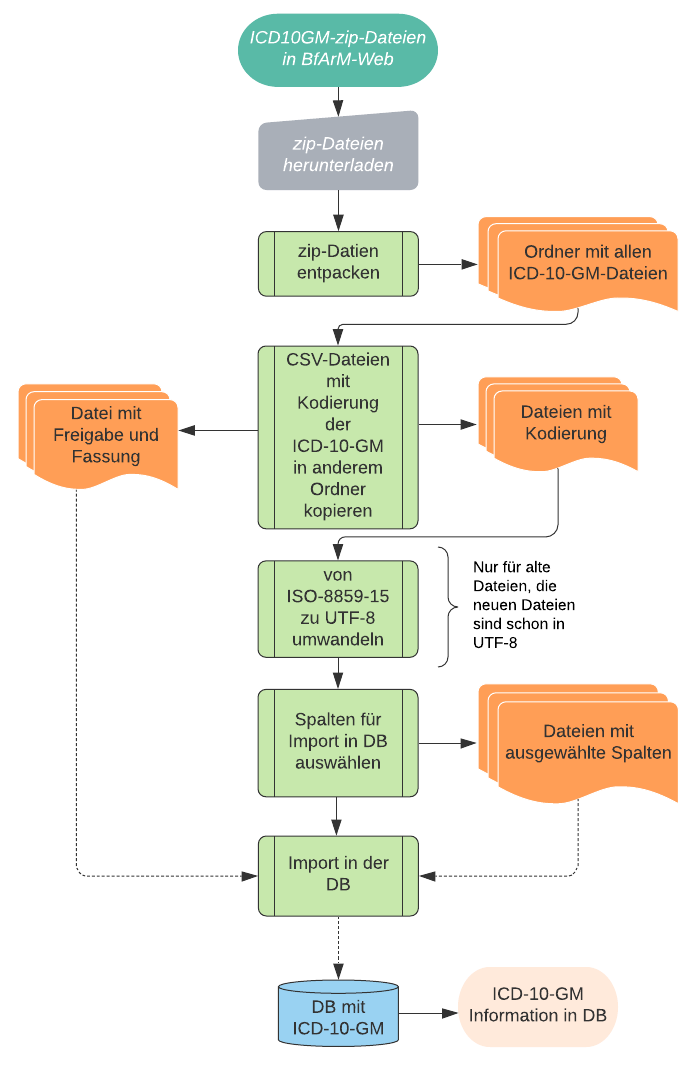
\includegraphics[height=14cm]{figures/etl}
	\caption[\acs{etl}-Strecke]{Flussdiagramm der \acs{etl}-Strecke für den Import der Information der \ac{icd10gm} aus den \ac{zip}-Dateien in der \ac{db}.}
	\label{fig:etl}
\end{figure} 

\subsection{Laden}

Am Ende das Skript \textsf{insert\_into\_db.sh} importiert die Information der \ac{csv}-Dateien in der Tabelle \textsf{kodes} der \ac{db}.	